% Ausarbeitung SAJ 
% FH Augsburg 
%
%
%
%
\documentclass[titlepage, 12pt,a4paper]{scrartcl}
%scrartcl
\usepackage[ngerman]{babel}
%\usepackage[latin1]{inputenc}
\usepackage[T1]{fontenc}
\usepackage{ucs}            % Eventuell benötigt
\usepackage[utf8x]{inputenc}

\usepackage{setspace}           % Paket fuer den Zeilenabstand
\onehalfspacing                 % Setzt den Zeilenabstand auf 1.5

\usepackage{graphicx}
\usepackage{listings}
\usepackage[hyphens]{url}
%\usepackage{breakurl}
\usepackage{hyperref}
\usepackage[usenames]{color}
\definecolor{light-gray}{gray}{0.90}
\usepackage[fixlanguage]{babelbib}
\usepackage{listings}
%\lstset{numbers=left, numberstyle=\tiny, numbersep=5pt}
%\lstset{language=Perl}
\lstloadlanguages{bash,XML,HTML, PHP, Python}
\selectbiblanguage{german}
\usepackage{makeidx}
%\usepackage{pifont}
\makeindex
%\usepackage{fancyhdr}
%\setlength{\headheight}{15.2pt}
%\pagestyle{fancy}


\author{Moritz Schächterle, Dominik Heimstädt \& Andrés Cuartas}
\title{- Studienarbeit Python - \\ WM-Tippspiel 2010 \\}
%\date{11-Dez-2007}

\pagestyle{myheadings}
\markright{Schaechterle, Heimstaedt \& Cuartas}
\lstset{
	inputencoding=utf8x,
	extendedchars=\true,
	language=Python,
	basicstyle=\tiny,
	keywordstyle=\bfseries\color{green},
	identifierstyle=,
	%commentstyle=\color{gray},	
	%stringstyle=\itshape\color{darkred},
	numbers=left,
	numberstyle=\tiny,
	stepnumber=1,
	breaklines=true,
	frame=none,
	showstringspaces=false,
	tabsize=4,
	backgroundcolor=\color{light-gray},
	captionpos=b,
	float=htbp,
	frameround=fttt
}


%\lstset{language=XML, stringstyle=\ttfamily, tabsize=2, basicstyle=\small, breaklines=true, backgroundcolor=\color{light-gray}, frameround=fttt}
%              
% WORKAROUND, damit lstlistoflistings funktioniert: 
% Quelle: http://www.komascript.de/node/477
%
\makeatletter% --> De-TeX-FAQ
\renewcommand*{\lstlistoflistings}{%
  \begingroup
    \if@twocolumn
      \@restonecoltrue\onecolumn
    \else
      \@restonecolfalse
    \fi
    \lol@heading
    \setlength{\parskip}{\z@}%
    \setlength{\parindent}{\z@}%
    \setlength{\parfillskip}{\z@ \@plus 1fil}%
    \@starttoc{lol}%
    \if@restonecol\twocolumn\fi
  \endgroup
}
\makeatother% --> \makeatletter 

\begin{document}

\maketitle
\newpage

\tableofcontents
\newpage

\section{Einführung}
Im Rahmen der Vorlesung „Internetprogrammierung mit Python“ ist eine
Studienarbeit zu erstellen. Aus mehreren zur Auswahl stehenden Arbeiten ist die
Wahl auf „Fußball-Tippspiel“ gefallen. Die Aufgabe darf im Team bearbeitet
werden mit maximal drei Gruppenmitgliedern. Aus aktuellem Anlaß wird die
Anwendug ein Fußball-WM Tippspiel mit der Möglichkeit auf die Begegnungen zu
tippen und für richtige Tipps, Differenz oder Tendenz Punkte zu erhalten. Die
Anwendung soll darüberhinaus noch ermöglichen einzusehen wieviele Punkte der
User momentan hat und auf welchen Platz er steht.

Bei der Überlegung zur Wahl geeigneter Werkzueuge zur Erstellung der Anwendung,
standen unter anderem Zope, Turbogears, Pylons und Django in der engeren
Auswahl.

Für die Auswahl geeigneter Werkzeuge sind folgende Punkte wichtig.
Arbeiten mit bekannten Techniken/Komponenten wie Python, mySQl,
ORM\footnote{Objekt-Relational Mapping}, HTML, JavaScript und Apache. 
Darüberhinaus sollte die Einarbeitungszeit nicht zu groß sein, da aus
Erfahrung, das Einarbeiten in neue Frameworks zeitaufwändig ist. Somit ist eine
gute Dokumentation ein weiterer wichtiger Punkt für die Auswahl.

Mit allen oben erwähnten Frameworks kommt man sicher schnell und einfach ans
Ziel. Letzenlich fiel die Wahl auf Django, da dieses Framework eine recht
schnelle Entwicklung für unsere Studienarbeit verspricht. Unter anderem sticht
die einfache Userverwaltung, der schnell zu konfigurierbare Adminbereich der
zur Verfügunggestellt wird, der OR-Mapper, das Templatesystem und der DRY: Don't
repeat yourself Ansatz. 

\section{Django}
Das Django Webframework eignet sich für die Erstellung von Webanwendungen. Es
folgt dem MVC\footnote{Model View Control} Muster. Wobei bei Django die Modelle
der Anwendung, die Objekte mit denen Django arbeitet mit Hilfe von OR-Mapping
in entweder mySQL, PostgreSQL, Oracle oder SQLite gespeichert werden können. So
wird die Datenpersistenz der Anwendung gewährleistet. Für die View sind
Templates zuständig, die mit Hilfe einer eigener Templatesprache konfiguriert
werden. Die Schnittstelle nach außen zum Server bieten die views (nicht zu
verwechseln mit der View), die die Kontrolle über die Anwendung bieten. Diese
beinhalten die Geschäftslogik und dienen als Verbindung zwischen den Modellen
und den Templates.


\section{Modelle}
Für die Anwendung stand zuerst die Erstellung der Klassen bzw. der
Datenbankmodelle die benötigt werden, um die vorgestellten Ziele erreichen zu
können. Folgende Klassen werden für die Anwendung benötigt. 

\begin{figure}[ht]
 \begin{center}
  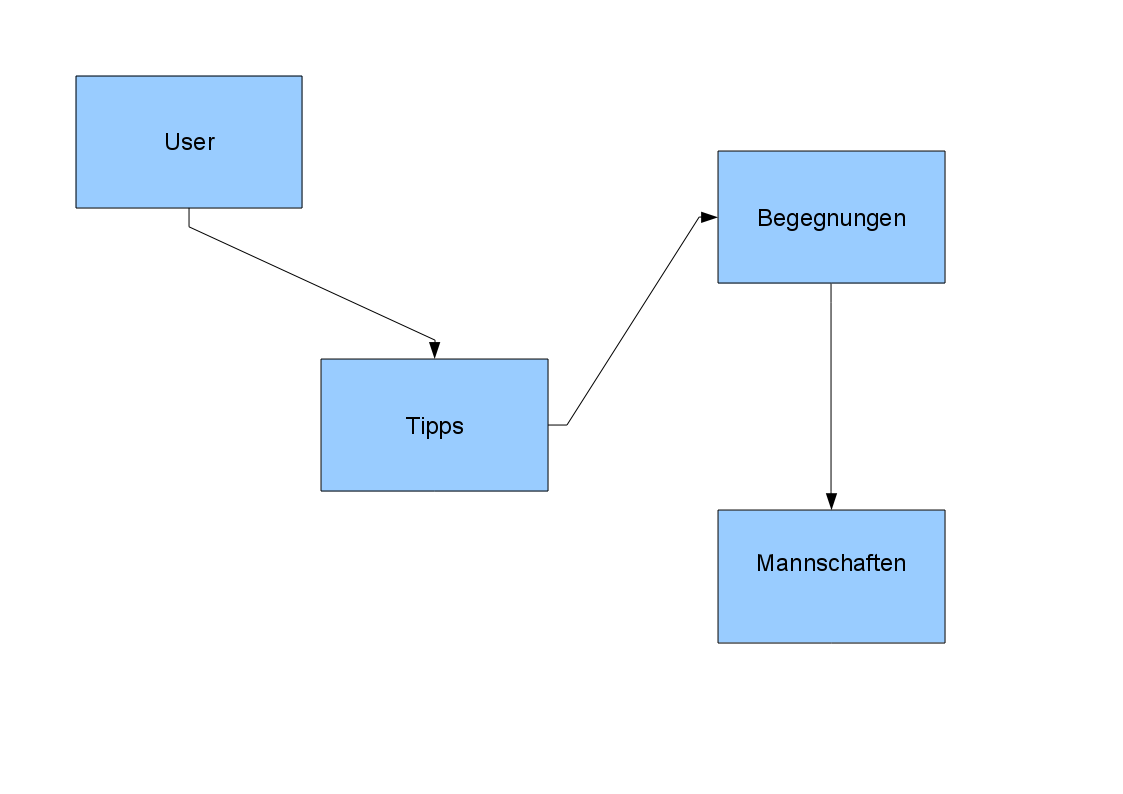
\includegraphics[scale=0.5]{pictures/klassen.png}
 \end{center}
 \caption{Benötigte Klassen}
 \label{klassen}
\end{figure}

Im Zentrum stehen die Tipps, welche die User abgeben können. Die Tipps setzen
sich zusammen aus den einzelnen Usern (Tipper) und den Spielbegegnungen. In
diesem Fall die Spiele der WM 2010. Weiterhin setzen sich diese aus Den
Mannschaften und weiteren Informationen, wie Spielzeit den Ergebnissen zusammen.
\\
\\

\begin{lstlisting}[caption=Modelle in Django]{modelleDjango}
class Tipps(models.Model):
    user = models.ForeignKey(User, unique=False)
    begegnung = models.ForeignKey(Begegnung, unique=False)
    
    toreHeim = models.IntegerField(max_length=2)
    toreGast = models.IntegerField(max_length=2)
    tippDatum = models.DateTimeField()
    
    def __unicode__(self):
        return u'%s %s' % (self.user, self.begegnung)
   
\end{lstlisting}

Mit Hilfe des eingebauten OR-Mappers in Django können die Tabellen aus den
vorher definierten Klassen als Tabellen in die Datenbank gespeichert werden.
Die Speicherung bzw. Synchronisation geschieht mit Django eigenen Boardmitteln.

\begin{lstlisting}[caption=Datenbanksynchronisation]{sync}
python manage.py syncdb
\end{lstlisting}

Damit python mit der Datenbank kommunizieren kann muss vorher ein
Datenbank-Connector installiert werden. Django unterstützt Oracle, PostgreSQL,
MySQL und SQLite. Die Installation des Connectors ist abhängig von der
Datenbank, die benutzt werden soll. Getestet wurden mySQL und PostgreSQL
hierbei bei der lokalen Entwicklung unter Ubuntu mySQL und auf dem
Produktionsserver Postgres. Bei der Speicherung und Auslesen der Daten erwies
sich mySQL toleranter, für den Produktionsserver mussten drei
Views\footnote{Django funktion} für PostgreSQL angepasst werden, weil
Exceptions von Django zurückgegeben wurden, die auf Probleme mit dem Speichern
und Auslesen von Daten zurückzuführen waren.

Mit Hilfe der Django eigenen Administrationsoberfläche, die einfach als
Applikation in der \emph{settings.py}\footnote{Datei beinhaltet alle
Umgebungsvariablen des Projektes} installiert werden kann, können leicht die
benötigten Einträge in die Datenbank geschrieben werden. Auch
\emph{Datetime-Felder} werden erkannt und es werden spezielle Widgets für die
Eintragung von Datenfeldern zur Verfügung gestellt. In dem Zusammenhang wurde
entschienden, die benötigten Informationen über Skripte, automatisch befüllen zu
lassen genaueres im Kapitel \ref{hilfsskripte} auf Seite \pageref{hilfsskripte}. 



\section{Views}
Die Geschäftslogik wird mit Hilfe der Views erstellt. Der Name ist hier etwas
irreführend, weil man View mit der Ausgabe, also HTML verküpft. Die View ist die
Schnittstelle, mit der die Anwendung mit dem Server/Client kommuniziert. Im
wmTippspiel wird beim Aufruf der Startseite, automatisch die dafür zuständige
View angesprochen. Diese führt Befehle aus, die ihre Ergenisse einem Template
übergeben kann. Das Template generiert aus den übergebenen Informationen
schließlich dann HTML, welches dem Server zur Weiterleitung an den Client zur
Verfügung gestellt wird.

In Django gibt es eine Kontrollinstanz, die ermöglicht, abhängig von der URL,
auf die verschiedenen Views der Seite zu verweisen. Einstellungen können in der
\emph{urls.py} gemacht werden. Mit Hilfe regulärer Audrücke wird die URL
untersucht. Der erste Ausdruck auf dem die URL passt, ermittelt und
die dahinterliegende View ausgeführt.

\begin{lstlisting}[caption=Auszug ursl.py]{urls.py}
urlpatterns = patterns('',
    (r'^$', index ),
    (r'^time/$', current_datetime ),
    (r'^displaymeta/$', display_meta ),
    #(r'^login/$', mylogin ),
    (r'^accounts/logout/$', 'django.contrib.auth.views.logout', {'next_page':'/'}),
    (r'^accounts/login/$', 'django.contrib.auth.views.login'),
    # Example:
    # (r'^wmTippspiel/', include('wmTippspiel.foo.urls')),

    # Uncomment the admin/doc line below and add 'django.contrib.admindocs'
    # to INSTALLED_APPS to enable admin documentation:
    # (r'^admin/doc/', include('django.contrib.admindocs.urls')),

    # Uncomment the next line to enable the admin:
    (r'^admin/', include(admin.site.urls)),
    
    (r'^tippspiel/', include('wmTippspiel.appWMTippspiel.urls')),
    
)
\end{lstlisting}

Im wmTippspiel wurde eine App\footnote{Eigenständiger Teil einer Webanwendung,
kann in verschiedenen Projekten eingebunden werden} erstellt und ausgelagert, so
kann die erstellte Applikation auch in anderen Internetseiten ohne viel Aufwand 
eingbunden werden.

\begin{lstlisting}
(r'^tippspiel/', include('wmTippspiel.appWMTippspiel.urls')),
\end{lstlisting}

Die appWMTippspiel bildet den Kern des wmTippspiel-Projekts. Daneben sind
weitere Applikationen, wie eine Registrierungs-Applikation
(siehe Kapitel \ref{registrierung}) denkbar, damit sich User bequem auf der
Seite registrieren können. Diese Applikation kann thematisch gut von der appWMTippspiel abgegrenzt werden und in anderen Projekten eingesetzt
werden. Was zu dem Don't repeat Yourself Gedankten Djangos passt.  

\section{Registrierung}\label{registrierung}
\section{Hilfsskripte}\label{hilfsskripte}

\section{Templates}
\section{Portierung auf Produktionsserver}
\section{Fazit}


\end{document}
